\documentclass{article}
\usepackage{graphicx}
\usepackage{float}
\usepackage{mathtools}

\title{ELEC 302-81\\ Lab 4\\ Transformers in Three Phase Circuits}
\date{\today}

\begin{document}

\maketitle

\begin{center}
  \begin{tabular}{lr}
    Date Performed: & February 11, 2013 \\
    Partners: & Rawley Dent \\
              & Charles Pittman \\
    Instructor: & Dr. Weatherford
  \end{tabular}
\end{center}

\pagebreak

\setlength\parindent{0pt}

\section{Purpose of Experiment}

The purpose of this experiment was to observe the basic principals of balanced
three-phase transformer circuits. Y-Y and Y-$\Delta$ connected transformer
banks were constructed separately to observe the differences, particularly in
their respective loads. Primary and secondary voltages, currents, and powers
were first calculated theoretically. Experimental values were then measured to
compare.

\section{Procedure}

\subsection{EMS Workstation Set-up}

At the Lab-Volt EMS workstation, the DAI 24-V supply was turned on, and the DAI
USB connector was connected between the EMS workstation and the {PC}. On the
LVDAM EMS application software, the metering windows for $E_1$, $E_2$, $I_1$,
$I_2$, $P_1$, 3$\phi$ power, $E_3$, $I_3$, and $E_1 + E_2 + E_3$ were
opened.  Under \emph{Options $\to$ Acquisition Settings}, the \emph{Sample
Window} dialog box was set to extended, and under \emph{View}, the
continuous refresh option was checked.

\subsection{The Three Phase Source}

\label{part1} The circuit represented by Figure~\ref{fig:circuit_01} was
constructed.  The main power switch was set to ON and the voltage control knob
adjusted to 120-V line-to-line. Both the installed analog EMS voltmeter and the
metering window were monitored for proper indications. The line voltages were
then measured and recorded in Table~\ref{tab:3phase_source}. The main power
switch was set to OFF and the voltage supply fully {CCW}. The circuit
represented by Figure~\ref{fig:circuit_02} was constructed. The main power
switch was set to ON and the voltage supply was adjusted to read 120-V
line-to-line. The installed analog EMS voltmeter was used for this since the
120-V were to be measured across voltage sources 4--5 only. The phase voltages
were then measured and recorded in Table~\ref{tab:3phase_source}.  The main
power switch was set to OFF and the voltage supply turned fully CCW.

\subsection{Y--Y Connected Transformer}

\label{part2} The circuit represented by Figure~\ref{fig:circuit_03} was
constructed.  The Y-connected load was (600 + j300)$\Omega$. The main power
switch was set to ON, and the voltage control knob adjusted to 120-V
line-to-line. Both the installed analog EMS voltmeter and the metering window
were monitored for correct voltage.  The values for primary and secondary line
voltage, primary and secondary line current, and primary input power were
measured and recorded in Table~\ref{tab:results}. A Fluke multimeter was used
to measure the RMS voltage across the load, labeled $E_4$, and recorded in
Table~\ref{tab:results}.  The main power switch was set to OFF and the voltage
control knob turned fully CCW.

\subsection{Y--$\Delta$ Connected Transformer}

\label{part3} The circuit represented by Figure~\ref{fig:circuit_04} was
constructed.  The Y-connected load was (600 + j300)$\Omega$. The main power
switch was set to ON, and the voltage control knob adjusted to 120-V
line-to-line. Both the analog EMS voltmeter and the metering window were
monitored for correct voltage. The values for primary and secondary line
voltage, primary and secondary line current, and primary input power were
measured and recorded in Table~\ref{tab:results}. A Fluke multimeter was used
to measure the RMS voltage across the load, labeled $E_4$, and recorded in
Table~\ref{tab:results}.  The main power switch was set to OFF and the voltage
control knob turned fully CCW.

\section{Results}
\subsection{The Three Phase Source}
\begin{table}[H]
  \centering
  \begin{tabular}{*{5}{c}}
    & \textbf{$E_1$} & \textbf{$E_2$} & \textbf{$E_3$} & \textbf{$E_1$+$E_2$+$E_3$} \\

    \hline

    \textbf{$V_{LL}$} & 120.4 & 117.1 & 116.3 & 0.998 \\
    \textbf{$V_{\phi}$} & 69.77 & 64.56 & 69.01 & 5.15 \\
  \end{tabular}
  \caption{Measured line and phase voltages for Part 1}
  \label{tab:3phase_source}
\end{table}

\begin{table}[H]
  \centering
  \begin{tabular}{*{7}{c}}
    & \multicolumn{2}{c}{\textbf{Primary}} &
    \multicolumn{2}{c}{\textbf{Secondary}} & \textbf{3$\phi$} & \textbf{Load} \\

    \textbf{Case} & \textbf{Voltage} & \textbf{Current} & \textbf{Voltage} &
    \textbf{Current} & \textbf{Input Power} & \textbf{Voltage} \\

    & $E_1$ V & $I_1$ A & $E_3$ V & $I_3$ A & $B$ W & $E_4$ V \\

    \hline
    Y--Y        & 121.2 & 0.112 & 119.5 & 0.097 & 19.8 & 58.4 \\
    Y--$\Delta$ & 120.1 & 0.151 & 68.4 & 0.055 & 4.7 & 32.4 \\
  \end{tabular}
  \caption{Measured Values}
  \label{tab:results}
\end{table}

\begin{table}[H]
  \centering
  \begin{tabular}{*{6}{c}}

    & \multicolumn{2}{c}{\textbf{Primary}}
    & \multicolumn{2}{c}{\textbf{Secondary}} & \textbf{Load} \\

    \textbf{Case} & \textbf{Line} & \textbf{Phase} & \textbf{Line} &
    \textbf{Phase} & \textbf{Phase} \\

    & V & V & V & V & V \\
    \hline

    Y--Y        & 120 & 69.3 & 120 & 11 & 69.3 \\
    Y--$\Delta$ & 120 & 69.3 & 69.3 & 11 & 40 \\
  \end{tabular}
  \caption{Computed Voltages}
  \label{tab:volt_comp}
\end{table}

\begin{table}[H]
  \centering
  \begin{tabular}{*{6}{c}}
    & \multicolumn{2}{c}{\textbf{Primary}}
    & \multicolumn{2}{c}{\textbf{Secondary}} & \textbf{Load} \\

    \textbf{Case} & \textbf{Line} & \textbf{Phase} & \textbf{Line} &
    \textbf{Phase} & \textbf{Phase} \\

    & A & A & A & A & A \\
    \hline

    Y--Y        & 0.1033 & 0.1033 & 0.1033 & 0.1033 & 0.1033 \\
    Y--$\Delta$ & 0.0596 & 0.0596 & 0.0344 & 0.0344 & 0.0344 \\
  \end{tabular}
  \caption{Computed Currents}
  \label{tab:curr_comp}
\end{table}

\begin{table}[H]
  \centering
  \begin{tabular}{*{4}{c}}
    \textbf{Case} & \textbf{Primary} & \textbf{Secondary} & \textbf{Load} \\

    & \textbf{Power} & \textbf{Power} & \textbf{Power} \\

    & W & W & W \\
    \hline

    Y--Y        & 19.20 & 19.20 & 19.2 \\
    Y--$\Delta$ & 6.40 & 6.4 & 6.4 \\
  \end{tabular}
  \caption{Computed Powers}
  \label{tab:pow_comp}
\end{table}

\begin{table}[H]
  \centering
  \begin{tabular}{*{7}{c}}
    & \multicolumn{2}{c}{\textbf{Primary}} &
    \multicolumn{2}{c}{\textbf{Secondary}} & \textbf{3$\phi$} & \textbf{Load} \\

    \textbf{Case} & \textbf{Voltage} & \textbf{Current} & \textbf{Voltage} &
    \textbf{Current} & \textbf{Input Power} & \textbf{Voltage} \\

    & $E_1$ V & $I_1$ A & $E_3$ V & $I_3$ A & $B$ W & $E_4$ V \\

    \hline
    Y--Y        & 0.99 & 7.77 & 3.03 & 0.42 & 6.49 & 18.7 \\
    Y--$\Delta$ & 0.17 & 77.2 & 37.3 & 1.21 & 8.36 & 23.46 \\
  \end{tabular}
  \caption{Percent Deviations}
  \label{tab:results}
\end{table}

\begin{table}[H]
  \centering
  \begin{tabular}{*{2}{c}}
    \textbf{Case} & \textbf{Efficiency} \\

    \hline

    Y--Y        & 54.29\% \\
    Y--$\Delta$ & 72.53\% \\
  \end{tabular}
  \caption{Transformer Efficiency}
  \label{tab:efficiency}
\end{table}



Equations Used:
\[\text{Transformer Efficiency} (\eta) = \frac{P_{out}}{P_\text{in}} * 100\% \]
\[\text{Percent Deviation} = \frac{\text{calculated data - lab data}}{\text{lab data}} * 100\%\]

\section{Conclusions} During Part 1: The Three-Phase Source, the three-phase
source line and phase voltages were measured. In Circuit 1, the three source
voltages are in a $\Delta$ connection, and hence the voltage values for each
phase are the same as the supply voltage 120-V line-to-line. When the voltages
are added together, they approximate 0 volts due to Kirchoff's voltage law. In
Circuit 2, the three source voltages are in a Y-connection, and hence the
voltage values for each phase are 1/$\sqrt{3}$ times the line voltage of 120-V.
When the voltages are added together, they approximate 0 volts, since the
connection is assumed to be balanced. When the Phasor Analyzer was analyzed on
the PC, it was confirmed that the phasors were equal with 120 degrees phase
shift for both the line and phase voltage measurements. The fact that the
addition of the phasors was not exactly zero was most likely due to the fact
that the voltage values measured were not exactly equal to each other.

When the transformer efficiencies for both connections were calculated, it was
found that the Y-$\Delta$ connection was more efficient than the Y-Y
connection. In the Y-$\Delta$ connection, the secondary $\Delta$ configuration
helped make the transformer bank more stable and thus more efficient. This was
most like due to the fact that a Y-$\Delta$ has no problem with third-harmonic
components in its voltages.

\section*{Circuits Tested}
\begin{figure}[H]
  \centering
  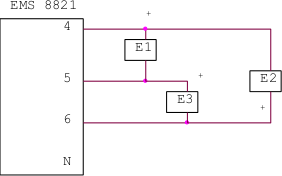
\includegraphics[width=.8\textwidth]{img/circuit_01}
  \caption{Circuit used to measure line voltages for Part 1}
  \label{fig:circuit_01}
\end{figure}

\begin{figure}[H]
  \centering
  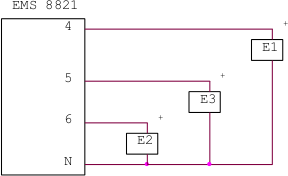
\includegraphics[width=.8\textwidth]{img/circuit_02}
  \caption{Circuit used to measure phase voltages for Part 1}
  \label{fig:circuit_02}
\end{figure}

\begin{figure}[H]
  \centering
  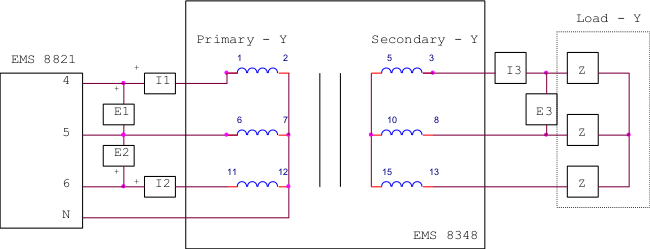
\includegraphics[width=.8\textwidth]{img/circuit_03}
  \caption{Y-Y connected three-phase transformer for Part 2}
  \label{fig:circuit_03}
\end{figure}

\begin{figure}[H]
  \centering
  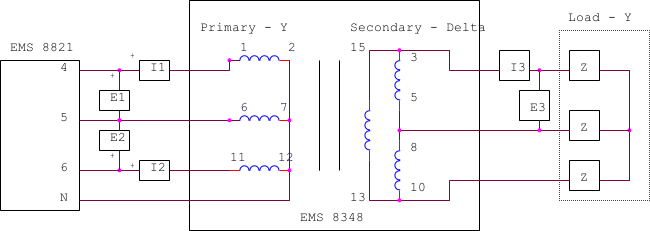
\includegraphics[width=.8\textwidth]{img/circuit_04}
  \caption{Y-$\Delta$ connected three-phase transformer for Part 3}
  \label{fig:circuit_04}
\end{figure}

\end{document}
